\newpage
\subsection{Caso d'uso UC3:  Registrazione Utente }
\label{UC3}
\begin{figure}[ht]
	\centering
	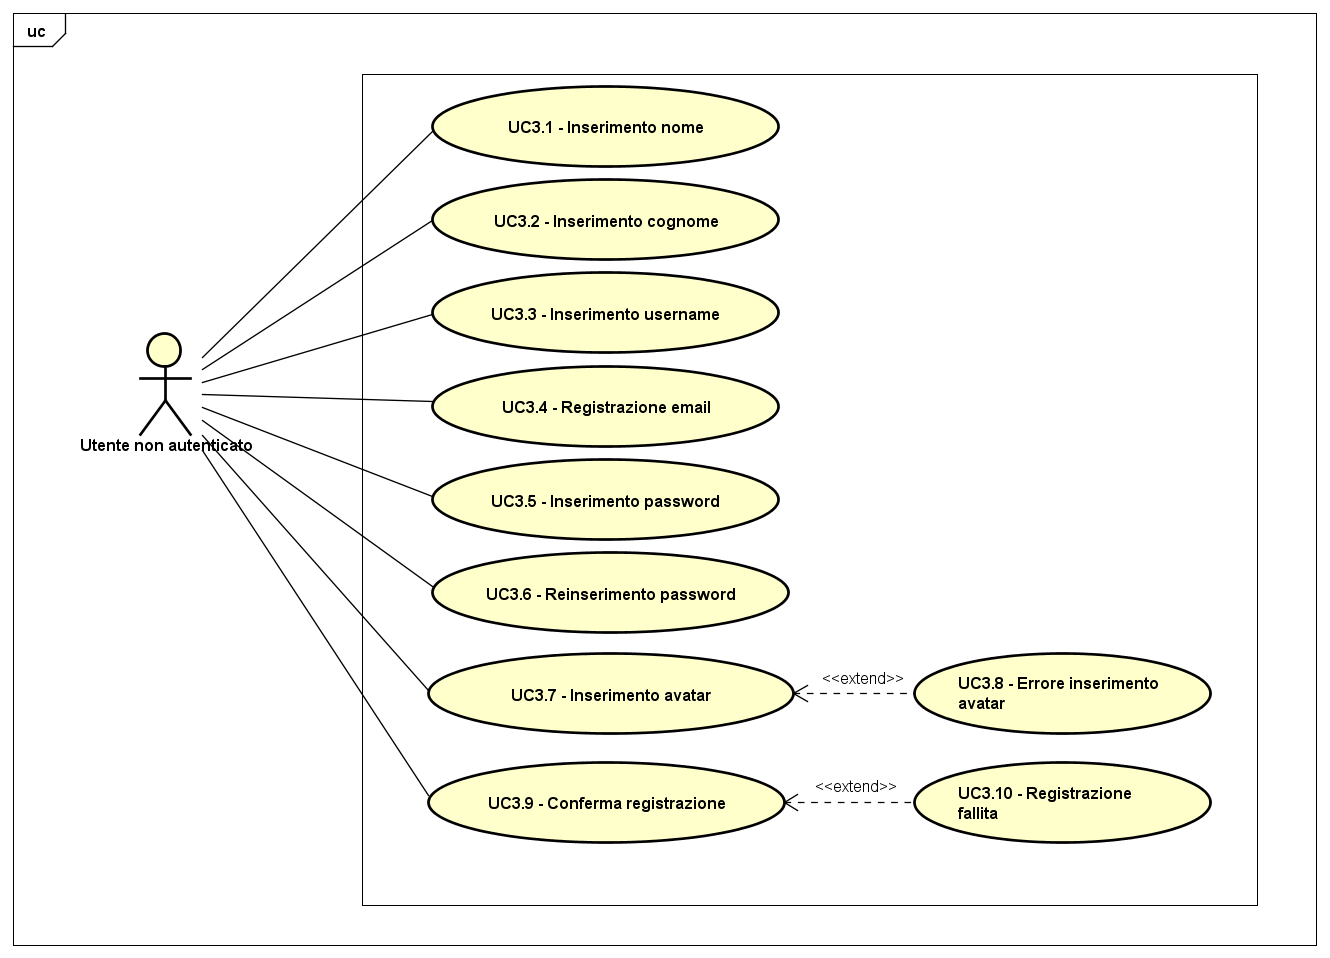
\includegraphics[scale=0.45]{UML/UC3.png}
	\caption{UC3: Registrazione Utente}
\end{figure}

\begin{longtable}{ l | p{11cm}}
	\hline
	\rowcolor{Gray}
	 \multicolumn{2}{c}{UC3 - Registrazione Utente} \\
	 \hline
	\textbf{Attori} & Utente Non Autenticato \\
	\textbf{Descrizione} & L'utente non autenticato inserisce le sue informazioni personali per potersi registrare all'applicazione web, così da poter successivamente effettuare il login ed evolversi in un utente autenticato.
	L'amministratore APIMarket, oltre alle funzionalità offerte all'utente autenticato, può
	visualizzare i dati di utilizzo delle API ed amministrare l'applicazione web.  \\
	\textbf{Pre-Condizioni} & L'utente ha scelto di registrarsi e l'applicazione web mostra la schermata di registrazione \\
	\textbf{Post-Condizioni} & L'utente si è registrato all'applicazione web \\
	\textbf{Scenario Principale} & \begin{enumerate*}[label=(\arabic*.),itemjoin={\newline}]
		\item L'utente non autenticato può inserire il proprio nome (UC3.1)
		\item L'utente non autenticato può inserire il proprio cognome (UC3.2)
		\item L'utente non autenticato può inserire il proprio username (UC3.3)
		\item L'utente non autenticato può inserire la propria email (UC3.4) 
		\item L'utente non autenticato può inserire la propria password (UC3.5)
		\item L'utente non autenticato può inserire la propria password per la conferma (UC3.6)
		\item L'utente non autenticato può confermare i dati inseriti, registrandosi all'applicazione web (UC3.7)
	\end{enumerate*}\\
	\textbf{Scenari Alternativi} & 
	\begin{enumerate*}[label=(\arabic*.),itemjoin={\newline}]
		\item L'utente non autenticato visualizza un errore e la registrazione non avviene (UC3.8)
	\end{enumerate*}\\
\end{longtable}